\subsection{Tarefa 04 -- Ajuste do Número de Neurônios por Camada}

\begin{comandoquestao}
	Objetivo: Avaliar como a quantidade de neurônios em cada camada oculta 
	influencia a capacidade de aprendizagem e a performance da rede neural. 
	Exploraremos diferentes arquiteturas para entender o impacto da 
	complexidade da 	rede.
\end{comandoquestao}

Foram realizados experimentos de treinamento com quatro diferentes 
configurações de neurônios nas camadas ocultas, mantendo o número de épocas 
constante em 10000. A primeira configuração com $[1, 5, 5, 5, 1]$ neurônios em 
cada camada resultou em uma perda de treinamento de $\approx 0,04058$. A 
segunda configuração com $[1, 10, 10, 10, 1]$ neurônios produziu uma perda de 
$\approx 0.04076$. A terceira configuração com $[1, 20, 20, 20, 1]$ neurônios 
resultou em 
uma perda de $\approx 0.04071$, e a quarta configuração com $[1, 50, 50, 50, 
1]$ neurônios 
teve uma perda de $\approx 0.04078$. As curvas de treinamento podem ser vistas 
na \cref{fig:tarefa04:curvas}

\begin{figure}[tbh]
	\centering
	\caption{Curvas de aprendizados para diferentes configurações da rede}
	\label{fig:tarefa04:curvas}
	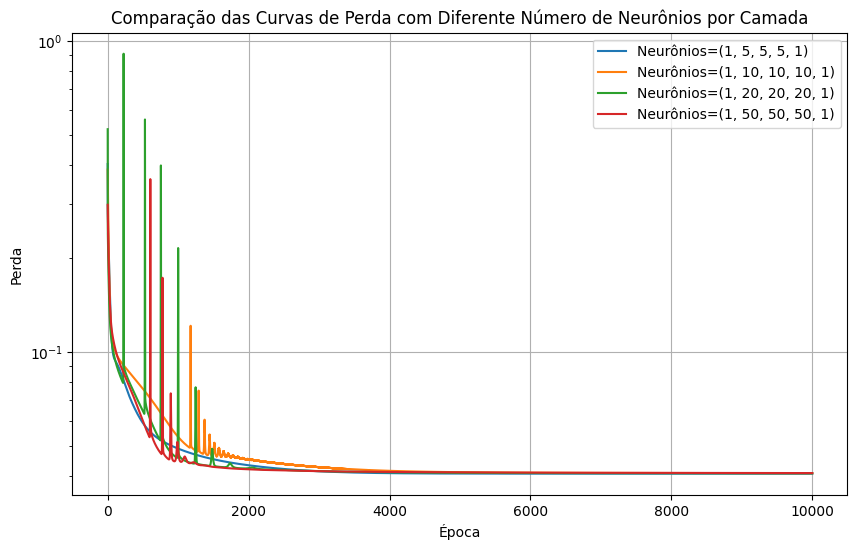
\includegraphics[width=0.7\linewidth]{./0803_imgs/png-241110-190844867-15619254497487317135.png}
\end{figure}

O efeito no tempo de treinamento para cada arquitetura pode ser visto na 
\cref{fig:tarefa04:tempo}. É importante notar que, conforme 
veremos mais adiante e com base na quantidade de dados disponível, não é 
necessário ter camadas muito densas com muitos neurônios.

\begin{figure}[tbh]
	\centering
	\caption{Tempo de treinamento de acordo com a arquitetura da rede}
	\label{fig:tarefa04:tempo}
	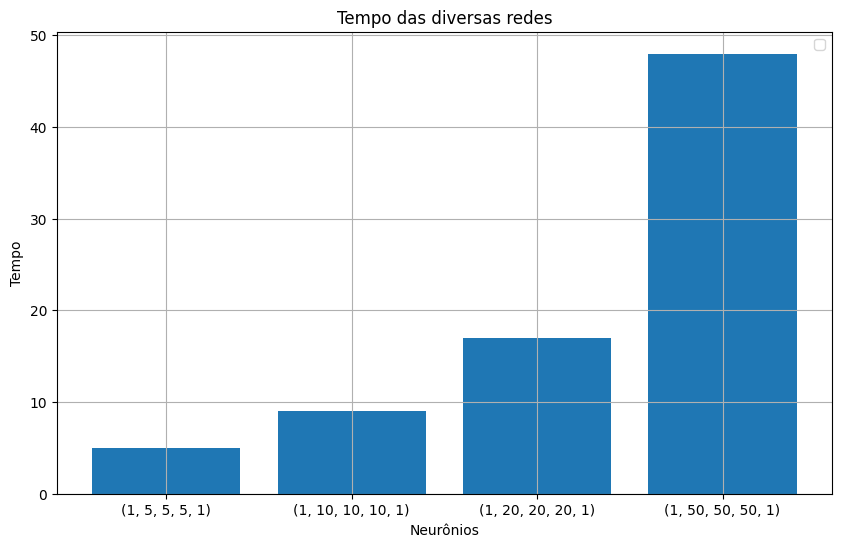
\includegraphics[width=0.7\linewidth]{./0803_imgs/png-241110-190809211-3985790047096570638.png}
\end{figure}

As predições das redes são mostradas nas 
\cref{fig:tarefa04:5:predicoes,fig:tarefa04:10:predicoes,fig:tarefa04:20:predicoes,fig:tarefa04:50:predicoes}
A configuração mais simples, com menos neurônios, apresenta uma boa 
convergência e uma curva de perda suave, sem muitas oscilações. Isso 
implica que, para este conjunto de dados específico, uma arquitetura de rede 
neural menos complexa pode ser suficiente para obter bons resultados.



\begin{figure}[htb]
	\centering
	\begin{minipage}{0.45\textwidth}
		\centering
		\caption{Configuração $[1, 5, 5, 5, 1]$}\label{fig:tarefa04:5:predicoes}
		
		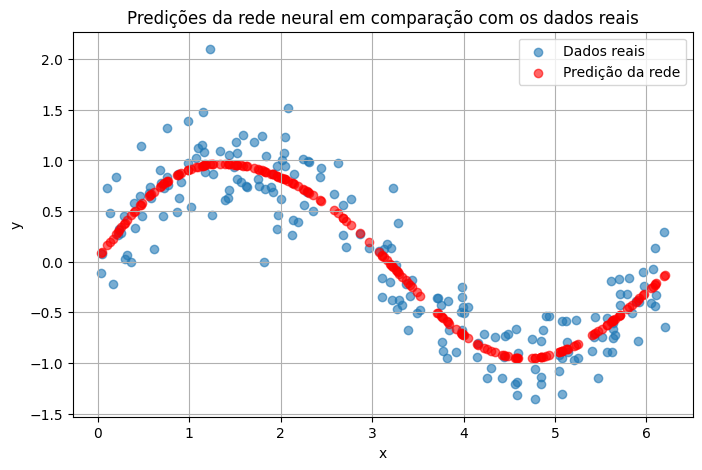
\includegraphics[width=\textwidth]{./0803_imgs/0052_tarefa04/png-241110-190441034-11876360900706154495.png}
		%\legend{Fonte: Gerado peloComando da atividade}
	\end{minipage}
	\hfill
	\begin{minipage}{0.45\textwidth}
		\centering
		\caption{Configuração $[1, 10, 10, 10, 
		1]$}\label{fig:tarefa04:10:predicoes}
		
		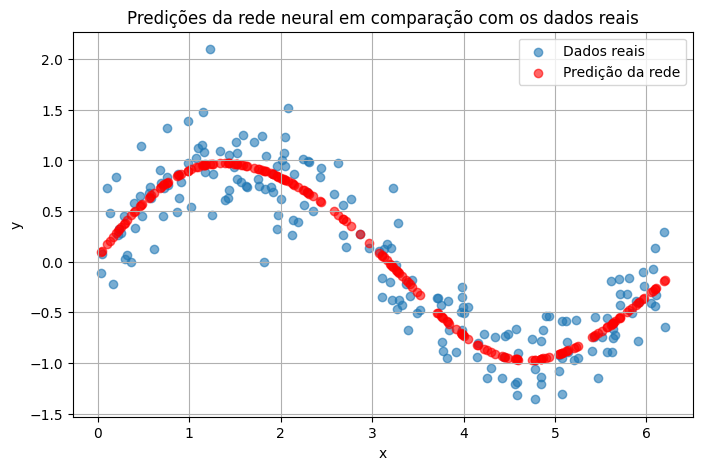
\includegraphics[width=\textwidth]{./0803_imgs/0052_tarefa04/png-241110-190600007-13238267918468901506.png}
		%\legend{Fonte: \citeonline[p. 24]{araujo2012}}
	\end{minipage}
	\vspace{2Ex}
	\begin{minipage}{0.45\textwidth}
		\centering
		\caption{Configuração $[1, 20, 20, 20, 
		1]$}\label{fig:tarefa04:20:predicoes}
		
		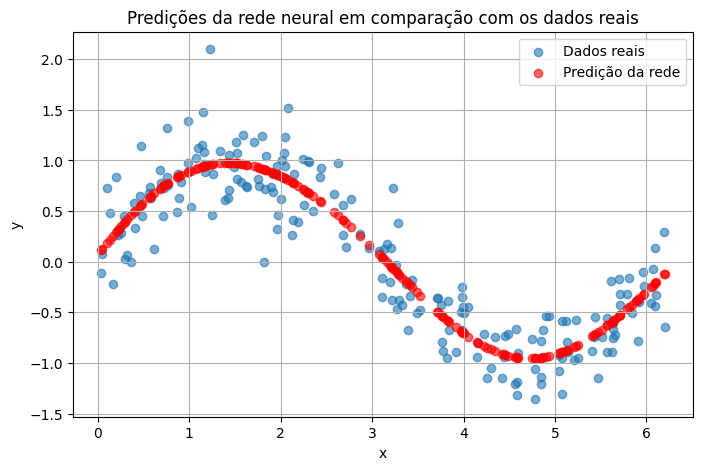
\includegraphics[width=\textwidth]{./0803_imgs/0052_tarefa04/png-241110-190633260-11858406457361919316.png}
		%		%\legend{Fonte: \citeonline[p. 24]{araujo2012}}
	\end{minipage}
	\hfill
	\begin{minipage}{0.45\textwidth}
		\centering
		\caption{Configuração $[1, 50, 50, 50, 
		1]$}\label{fig:tarefa04:50:predicoes}
		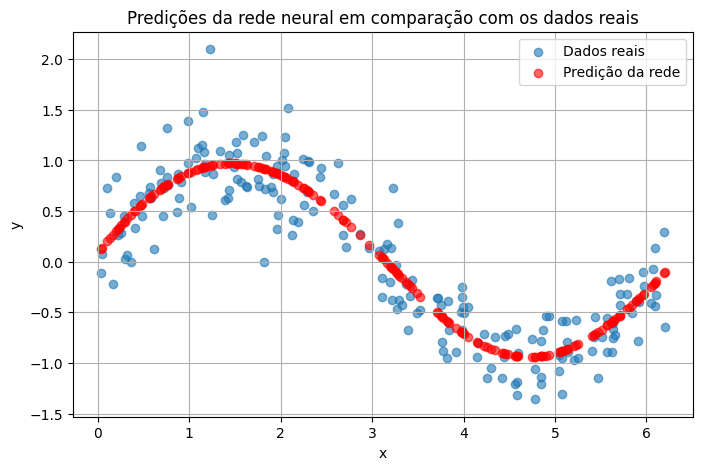
\includegraphics[width=\textwidth]{./0803_imgs/0052_tarefa04/png-241110-190650933-14380430249431153222.png}
		%\legend{Fonte: \citeonline[p. 24]{araujo2012}}
	\end{minipage}
\end{figure}


Em resumo, esta análise destaca a importância de considerar a complexidade da 
arquitetura da rede neural em relação à quantidade de dados disponíveis. Em 
alguns casos, uma rede neural mais simples pode convergir bem e fornecer 
resultados comparáveis a redes mais profundas e complexas. A escolha da 
arquitetura ideal depende dos dados específicos e dos objetivos do problema em 
questão.

